\documentclass[12pt]{article}

\usepackage[margin=1in]{geometry} 
\usepackage{amsmath,amsthm,amssymb,amsfonts}
\usepackage{graphicx}
\usepackage{listings}
\usepackage{color}
\usepackage{caption}
\usepackage{subcaption}

\definecolor{mygreen}{rgb}{0,0.6,0}
\definecolor{mygray}{rgb}{0.5,0.5,0.5}
\definecolor{mymauve}{rgb}{0.58,0,0.82}

\lstset{basicstyle=\footnotesize ,
tabsize=4,
commentstyle=\color{mygreen},
numbers=left,
numbersep=5pt,
numberstyle=\tiny\color{mygray},
rulecolor=\color{black},
stringstyle=\color{mymauve}}

\begin{document}

\title{CS 5785 Applied Machine Learning, Homework 4}
\author{Wen Guo (wg264), Roger Wang (rw575)}
\maketitle

{\parindent0pt
\section*{Programming Exercises}
\subsection*{Question 1}
\subsubsection*{(a)}
I found a famous image of our president Trump.

\medskip
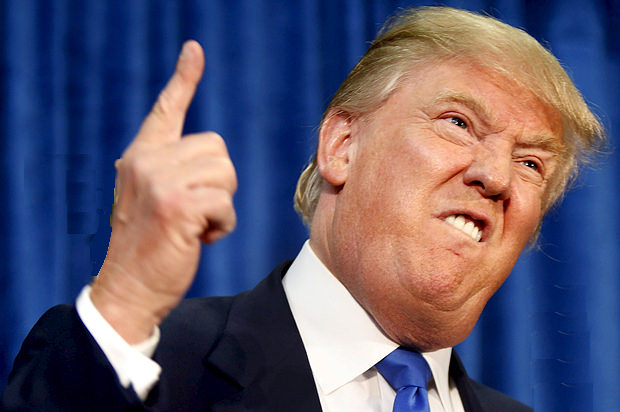
\includegraphics[scale=0.2]{P1/Trump.jpg}

\subsubsection*{(b)}
The size of the image is 412*620=255440 pixels. Each pixel is a list of three values representing red, green, blue value of the color. $[r,g,b]\ (0\leqslant r \leqslant 255,0\leqslant g \leqslant 255,0\leqslant b \leqslant 255)$. I randomly choose 3000 coordinates from all possible coordinates. ($(x,y) \quad \forall x\in \{0,1,2,...,411\}, \forall y\in \{0,1,2,...,619\} $) I didn't do any preprocessing for the input, because the coordinates are independently identically distributed random variables and each node of the random forests is a random sample of features. There is no need to perform mean subtraction, standardization, or unit-normalization.

\subsubsection*{(c)}
I reshape the flattened predicted list back to a 412*620 matrix to display the graph. Each value in the matrix is a [r,g,b] list. There is no need to do any preprocessing for the output, because cv2.imwrite accepts float value for r,g,b.

\subsubsection*{(d)}
I use sklearn.ensemble.RandomForestRegressor to train and predict each pixel's color. I use the default tree depth which will split until all leaves are pure or there are less than 2 samples in a group. The default number of decision trees are 100.

\medskip

\includegraphics[scale=0.2]{P1/RF_Trump.jpg}

\subsubsection*{(e)}
\textbf{i.}

Holding the number of decision tree constant, as the depth increases, there are more color regions. When decision tree's depth is 1, there are 2 leaf nodes in the decision tree. Each leaf node represents one outcome (one group of color). Therefore, there are 2 color regions. When decision tree's depth is 2, there are 4 leaf nodes. Therefore, there are 4 color regions. Decision tree with depth 5 has $2^5=32$ color regions. Decision tree with depth 10 has $2^{10}=1024$ color regions. Decision tree with depth 15 has $2^{15}=32768$ color regions.

\medskip
The following images all have single decision tree and the depth of decision tree are 1, 2, 3, 5, 10, 15.


\includegraphics[scale=0.12]{P1/RF_Trump_depth1trees1.jpg}

\includegraphics[scale=0.12]{P1/RF_Trump_depth2trees1.jpg}

\includegraphics[scale=0.12]{P1/RF_Trump_depth3trees1.jpg}

\includegraphics[scale=0.12]{P1/RF_Trump_depth5trees1.jpg}

\includegraphics[scale=0.12]{P1/RF_Trump_depth10trees1.jpg}

\includegraphics[scale=0.12]{P1/RF_Trump_depth15trees1.jpg}

\medskip
\textbf{ii.}

Holding the depth of decision tree constant, as the number of decision tree increases, the color region boundary becomes smoother. When the number of decision tree is 1, there is only one tree deciding the boundary. Therefore, the boundary is 1 sharp line. When the number of decision tree is 3, there are three trees drawn from random samples deciding the pixel color. Given the bias of each tree is the same, the variance will be smaller. Therefore, the boundary will be smoother and the whole image is more detailed.

\medskip
The following images all have tree depth 7 and the number of decision trees are 1, 3, 5, 10, 100.


\includegraphics[scale=0.15]{P1/RF_Trump_depth7trees1.jpg}

\includegraphics[scale=0.15]{P1/RF_Trump_depth7trees3.jpg}

\includegraphics[scale=0.15]{P1/RF_Trump_depth7trees5.jpg}

\includegraphics[scale=0.15]{P1/RF_Trump_depth7trees10.jpg}

\includegraphics[scale=0.15]{P1/RF_Trump_depth7trees100.jpg}

\medskip
\textbf{iii.}

Because the sample has 3000 random points, there are 3000 color regions in the image. Every pixel's color is decided by the closest sample point's color. Each sample point forms a polygon. Each line of the polygon is the middle cut line from the sample point to its nearby sample points.

\medskip
The following graph is 1NN.


\includegraphics[scale=0.2]{P1/1NN_Trump.jpg}

\medskip
\textbf{iv.}

As the depth and number of trees increase, the image becomes more realistic and closer to the original image. However, the change becomes smaller when the tree depth and the number of trees are large value.

depth: 10, 20, 40

trees: 20, 40, 80


\includegraphics[scale=0.2]{P1/RF_Trump_depth10trees20.jpg}

\includegraphics[scale=0.2]{P1/RF_Trump_depth20trees40.jpg}

\includegraphics[scale=0.2]{P1/RF_Trump_depth40trees80.jpg}

\subsubsection*{(f)}
\textbf{i.}

Denote the coordinate as (x,y) where x is the image's row index and y is the image's column index. The decision rule is $x \leqslant a\ (0\leqslant a \leqslant 899)$ or $y \leqslant b\ (0\leqslant b \leqslant 603)$. For the image with max depth of one and one decision tree. The rule for the split point is $x \leqslant 479$. If $x \leqslant 479$, the gray-scale value is 102, otherwise the gray-scale value is 42.

\medskip
\textbf{ii.}

The patches of color are rectangles. Because the decision rule is based on the x or y coordinate, the boundary will be a horizontal or vertical line and the boundary will form a rectangle. For the most of the smallest rectangles, they are arranged as part of a large rectangle with either the same height or the same width.

\medskip
\textbf{iii.}

Denote the depth of the decision tree as d. If the forest contains a single decision tree, there are $2^d$ patches of color. The number of tree nodes is $2^d$. Each tree node is a color region.

\medskip
\textbf{iv.}

Denote the depth of the decision tree as d. The number of colors as c. If the forest contains n decision tree, then $2^d \leqslant c \leqslant 2^d+(2^{d}-1)\cdot(n-1)$. Each decision tree has $2^d-1$ boundaries (non-leaf node). Every increase in the number of decision tree will increase the number of color region at most $2^d-1$. The decision tree's boundary maybe the same as other tree's, so at most $2^d-1$.

\subsection*{Question 2}
\subsubsection*{(a)}
After random sampling, for the training set, we got 300 "MM" class and around 500 "CH" class. For the test set, we got around 105 "MM" class and 165 "CH" class. 

\begin{center}
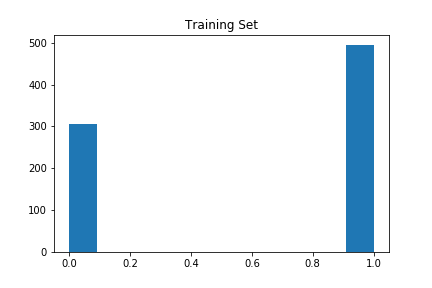
\includegraphics[scale=0.5]{P2/3a_class_fraction_training.png}
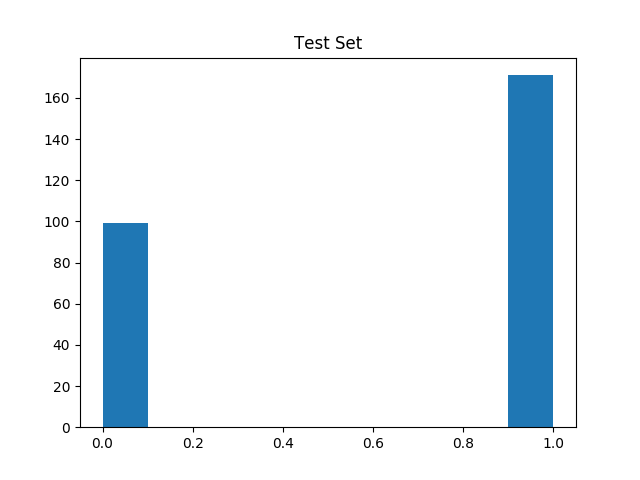
\includegraphics[scale=0.5]{P2/3a_class_fraction_test.png}
\end{center}


\subsubsection*{(b)}
The SVM classfier learns a model $ f(X)= \beta^T X + \beta_0 $ that minimize $\Vert \beta \Vert + C\cdot\Sigma_i^{N} \xi_i $ . In essence, the sign of the fitted value determines on which side of the decision boundary the observation lies. If the fitted value exceeds zero then the observation is assigned to one class, and if it is less than zero than it is assigned to the other. 

For the learned coefficients, 
the number of support vectors for each class is [305 309].
 The constants in decision function is [-1.55824063]. The weights assigned to the features is: \newline
[ 0.00313619  0.10952847 -0.03483193  0.04412031  0.01375094 -0.16467846
   0.07207978 -0.27        1.01626556  0.20879877 -0.04858287  0.25738164
  -0.01682384 -0.07617903  0.00742896  0.07895224]
 
\subsubsection*{(c)}
Because of the random sampling, the error rates varies. In one of our tries, the training error rate is 0.22 and the test error rate is 0.21. 

\subsubsection*{(d)}
The cost-accuracy plot shows that the test accuracy is the highest when C=0.07. According to the one-stderr error, the best C is 0.06. 

\begin{center}
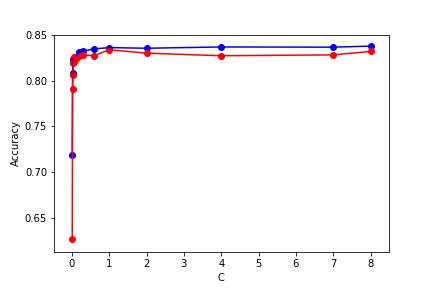
\includegraphics[scale=0.8]{P2/cross_validation_linear.png}
\end{center}

\subsubsection*{(e)}
When C=0.06, the training error rate is 0.1687; the test error rate is 0.1963. 


\subsubsection*{(f)}
A smaller $\gamma$ means greater $\sigma$ and larger bandwidth. Larger RBF kernel bandwidths produce smoother feature space mappings and smoother decision boundaries, which means a simpler model. 


\subsubsection*{(g)}
Using C=0.01, the training and test accuracy is 0.615 and 0.596. The learned coefficients include: \newline
Number of support vectors for each class: [308 319] \newline
Constants in decision function. [0.96515056]

The red line is the test accuracy plot. According to one-standard-error rule, the appropriate gamma should be 0.4. 
\begin{center}
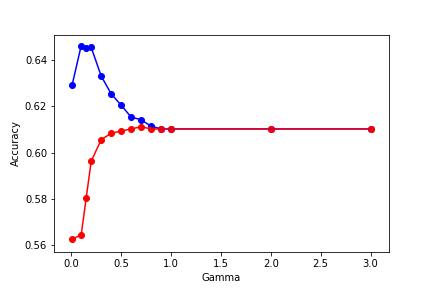
\includegraphics[scale=0.8]{P2/cross_validation_rbf_gamma.png}
\end{center}

\subsubsection*{(h)}
According to one-standard-error rule, the appropriate gamma should be 0.5 for the polynomial kernel. 

\subsubsection*{(i)}
According to our results, the linear kernel with C=0.06 gives the best results. 

\subsection*{Question 3}
\subsubsection*{(a)}
This network has 7 layers. Each layer has 20 neurons. It uses ReLU (rectified linear units) activation function. $x = max(0, x)$

\subsubsection*{(b)}
Loss measures the inconsistency between predicted value ($\hat{y}$) and the actual label(y). It is a non-negative value, where the robustness of model increases along with the decrease in loss function's value. In this case, the actual loss function is L2 loss function. $L = \sum_{i=1}^n(y^i-\hat{y}^i)^2$

\subsubsection*{(c)}
The loss at 5002 iterations is 0.005765.

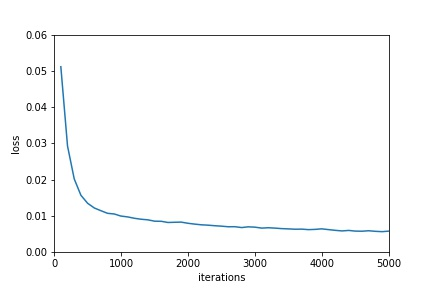
\includegraphics[scale=1]{P3/c.jpg}

\subsubsection*{(d)}
I cut the learning rate by half at 1002, 2002, 3002, 4002 iterations. The final learning rate is $0.01 \div 2^4 = 0.000625$ and the loss at 5001 iterations is 0.003753. Because $0.003753 < 0.005765$, the neural network converges to a lower loss function.

\subsubsection*{(e)}
7 layers, the loss at 5002 iterations is 0.005765.

6 layers, the loss at 5002 iterations is 0.005509.

5 layers, the loss at 5002 iterations is 0.005775.

4 layers, the loss at 5002 iterations is 0.006371.

3 layers, the loss at 5002 iterations is 0.007057.

2 layers, the loss at 5002 iterations is 0.011695.

1 layers, the loss at 5003 iterations is 0.025877.

\medskip
I can drop three layers before the accuracy drops
below a useful value. After I drop the four layers, the image quality drops noticeably.

\medskip
20 units, the loss at 5002 iterations is 0.005765.

18 units, the loss at 5002 iterations is 0.006277.

16 units, the loss at 5002 iterations is 0.005721.

14 units, the loss at 5002 iterations is 0.006353.

12 units, the loss at 5002 iterations is 0.007078.

11 units, the loss at 5002 iterations is 0.006928.

10 units, the loss at 5001 iterations is 0.007451.

\medskip
I can reduce up to 9 hidden units before the image quality drops noticeably.

\subsubsection*{(f)}
7 layers, the loss at 5002 iterations is 0.005765.

8 layers, the loss at 5002 iterations is 0.005395.

9 layers, the loss at 5002 iterations is 0.005235.

\medskip
There is no obvious improvement and the training speed is significantly slower.

\section*{Written Exercises}
\subsection*{Question 1}
\subsubsection*{(a)}
If this split is replaced by a leaf labeled with the more frequent class, for the left branch, the training mistakes would be $\min \lbrace p_{1}, n_{1} \rbrace $. 

\begin{eqnarray*}
\text{left branch \# of mistake} &=& \min \lbrace p_{1}, n_{1} \rbrace \\
&=& (p_{1} + n_{1}) \frac{\min \lbrace p_{1}, n_{1} \rbrace}{(p_{1} + n_{1})} \\
&=& (p_{1} + n_{1}) \min\{\frac{p_1}{p_1+n_1},\frac{n_1}{p_1+n_1}\} \\
&=& (p_{1} + n_{1}) \min\{\frac{p_1}{p_1+n_1},\frac{1-p_1}{p_1+n_1}\} \\
&=& (p_{1} + n_{1})\cdot f(\frac{p_{1}}{p_{1}+n_{1}})
\end{eqnarray*}

Similarly,

\[
\text{left branch \# of mistake} = \min \{p_{2}, n_{2}\} = (p_{2} + n_{2})\cdot f(\frac{p_{2}}{p_{2}+n_{2}})
\]

Therefore,

\[
\text{total training mistakes} = (p_{1} + n_{1})\cdot f(\frac{p_{1}}{p_{1}+n_{1}}) + (p_{2} + n_{2})\cdot f(\frac{p_{2}}{p_{2}+n_{2}}) = \text{weighted impurity}
\]

Thus, using the min-error impurity is equivalent to growing the tree greedily to minimize training error.

\subsubsection*{(b)}
If $a_1$ = 0, $p(+)=\frac{2}{4}$, $p(-)=\frac{2}{4}$.

If $a_1$ = 1, $p(+)=\frac{1}{6}$, $p(-)=\frac{5}{6}$.

If $a_2$ = 0, $p(+)=\frac{1}{4}$, $p(-)=\frac{3}{4}$.

If $a_2$ = 1, $p(+)=\frac{2}{6}$, $p(-)=\frac{4}{6}$.

If $a_3$ = 0, $p(+)=\frac{3}{7}$, $p(-)=\frac{4}{7}$.

If $a_3$ = 1, $p(+)=\frac{0}{3}$, $p(-)=\frac{3}{3}$.

\medskip
Gini impurity for $a_1 = \frac{4}{10}\cdot(1-(\frac{1}{2})^2-(\frac{1}{2})^2)+\frac{6}{10}\cdot(1-(\frac{1}{6})^2-(\frac{5}{6})^2)=0.3667$

\medskip
Gini impurity for $a_2 = \frac{4}{10}\cdot(1-(\frac{1}{4})^2-(\frac{3}{4})^2)+\frac{6}{10}\cdot(1-(\frac{2}{6})^2-(\frac{4}{6})^2)=0.4167$

\medskip
Gini impurity for $a_3 = \frac{7}{10}\cdot(1-(\frac{3}{7})^2-(\frac{4}{7})^2)+\frac{3}{10}\cdot(1-(\frac{0}{3})^2-(\frac{3}{3})^2)=0.3429$

Because $a_3$ has the smallest Gini impurity, choose $a_3$.

\medskip
Min-error impurity for $a_1 = 2 + 1 = 3$.

\medskip
Min-error impurity for $a_2 = 1 + 2 = 3$.

\medskip
Min-error impurity for $a_1 = 3 + 0 = 3$.

Because $a_1,a_2,a_3$ has the same min-error impurity, they can all be chosen as the split.

%Gini impurity is a measurement of the likelihood of an incorrect classification of a new instance of a random variable, if that new instance were randomly classified according to the distribution of class labels from the data set. The formula to calculate Gini impurity is: 
%
%\begin{center}
%$I_{G} = p_{+}(1-p_{+}) + p_{-}(1-p_{-})$
%\end{center}
%
%The further away from $p=0.5$, the lower the Gini impurity. 
%\begin{center}
%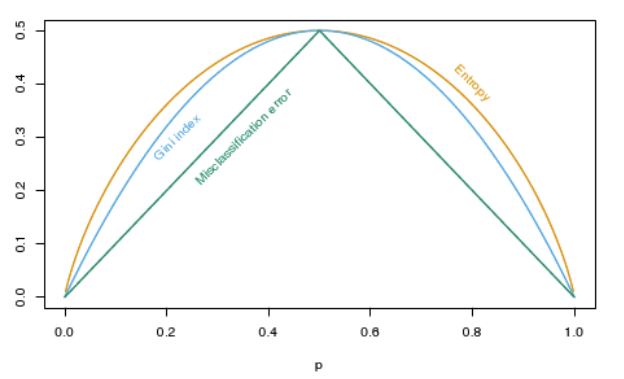
\includegraphics[scale=0.5]{impurity_measures.png}
%\end{center}
%
%if min-error impurity is used, 
%for $a_{1}$ split, the training error is 3;
%for $a_{2}$ split, the training error is 5;
%for $a_{1}$ split, the training error is 4. 
%Based on our discussion in (2), minimizing training errors is equivalent to minimizing min-error impurity. Thus, we should choose $a_{1}$ split.  
%
%Gini impurity for 

\subsubsection*{(c)}
If $\min\{p_1, n_1\} + \min\{p_2, n_2\} < \min\{p, n\}$,
then it must satisfy one of the two conditions: 
$p_1 < n_1$ and $p_2 > n_2$;
$p_1 > n_1$ and $p_2 < n_2$.

\subsubsection*{(d)}
The min-error impurity is not suitable for growing decision trees, because it is likely to get the same min-error impurity for lots of features and after each split, the weighted min-error impurity is not likely to change. The decision trees won't be accurate.

\subsection*{Question 2}

For each sample, the probability of a sample in the training set not appearing in the bootstrap replicate is: 
\begin{center}
$P(X_{i}=0) =(\frac{N-1}{N})^N  = {(\frac{1}{\frac{N}{N-1}}})^{N}= \frac{1}{  ({1 + \frac{1}{N-1}} )^{N} }$
\end{center}

\begin{center}
$ \lim_{N\to\infty} P(X_{i}=0) = e^{-1}$
\end{center}

According to the properties of Bernoulli distribution, the expected number of samples not appearing in the bootstrap replicate  is: 
\begin{center}
$E(X)= N\cdot P(X_{i}=0) = Ne^{-1} $
\end{center}

which means around 36.8 percent of the training data will not appear in the boostrap replicate. 

\subsection*{Question 3}
\subsubsection*{(a)}
The solid line in the following graph is the maximum separating hyper plane. 
\begin{center}
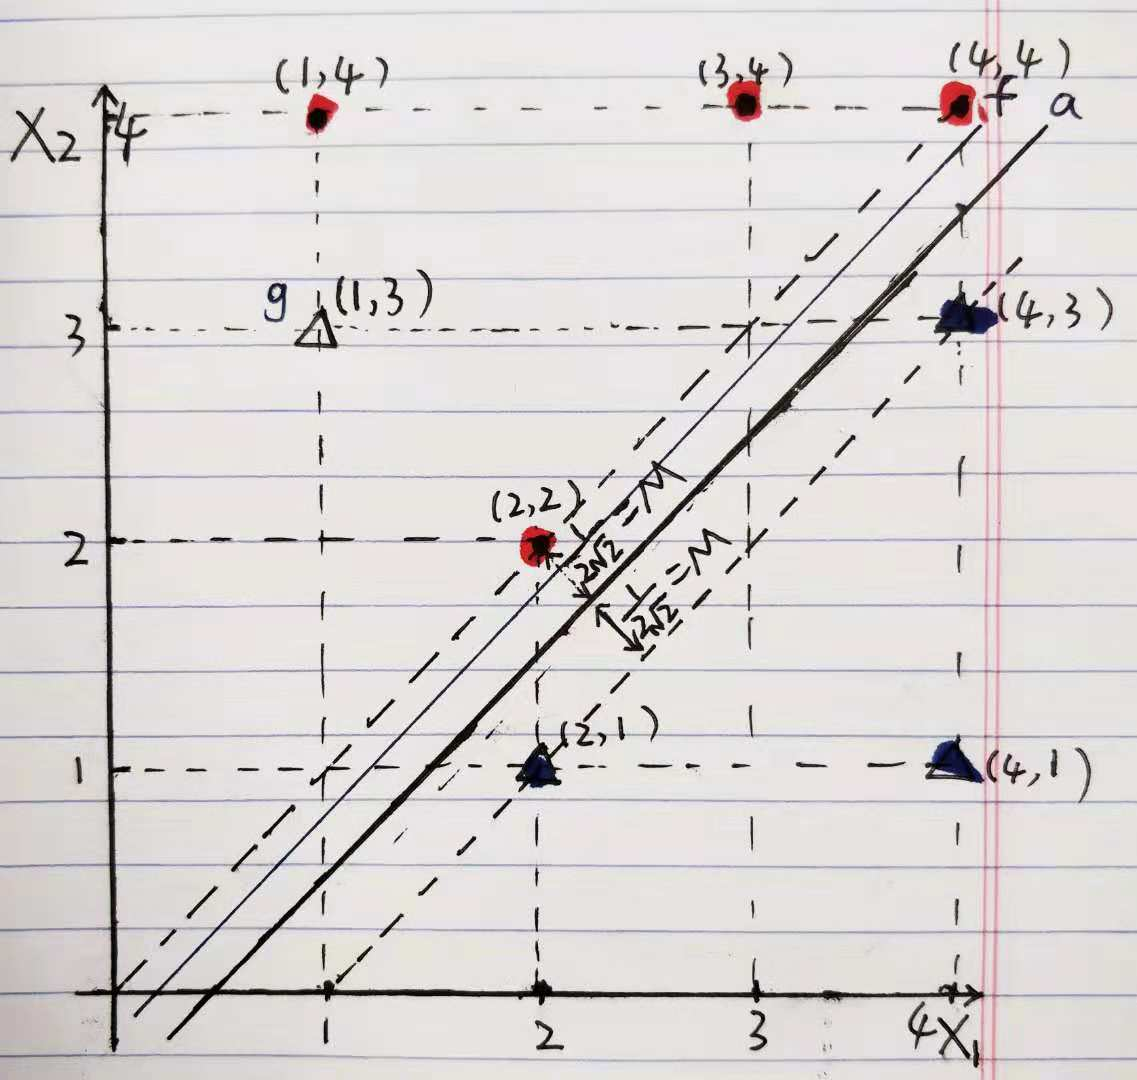
\includegraphics[scale=0.3]{max_margin_classifier.jpg}
\end{center}

\subsubsection*{(b)}
The classification rule is that, any observation that make $X_{1}-X_{2}-0.5 > 0$ should be classified as "Blue". Otherwise, "Red". 

That is, the values for $\beta$ are: 
\begin{center}
$\beta	_{0} = -0.5; \beta_{1} = 1; \beta_{2} = -1$
\end{center}

\subsubsection*{(c)}
The margin for the maximum hyper plane is: 

$2M=\frac{2}{|| \beta ||}=\frac{2}{2\sqrt{2}}=\frac{\sqrt{2}}{2}$

\subsubsection*{(d)}
Support vectors are the data points that lie closest to the decision surface. For this observations, the 4 support vectors are (2,2), (4,4), (2,1) and (4,3). 

\subsubsection*{(e)}
Because the seventh observation is not the support vector, its slight movement will not affect the hyper plane. 

\subsubsection*{(f)}
One hyper plane that separates the data, but is not the maximum-margin separating hyper plane could be $X_{1}-X_{2}-0.2 =0 $

\subsubsection*{(g)}
An additional observation of (1,3) "Blue" would make the two classes no longer separable by a hyper plane.
}
\end{document}